\chapter{Application of Machine Learning Algorithms}
\label{chap:four}

\section{Repository and Environment Structure}
\section{Data Exploration}
This section is focused on exploration of the analyzed loan dataset, particularly on dataset description, distribution analysis and association analysis, in order to infer potential valuable insights and hypotheses which can be used in the preprocessing or modelling part.

\subsection{Dataset Description}
The analyzed dataset pertains to the HMEQ dataset which contains loan application information and default status of 5,960 US home equity loans. Such dataset was acquired from Credit Risk Analytics.

As can be seen in \autoref{tab:dataset}, the dataset contains 12 columns, 11 features and 1 target variable \texttt{BAD} indicating whether the loan was in default (\texttt{1}) or not (\texttt{0}). 
Amongst the 11 features, there are 9 numeric features and 2 categorical features, namely \texttt{REASON} which contains 2 categories - Debt consolidation (\texttt{DebtCon}) and Home improvement (\texttt{HomeImp}), and \texttt{JOB} which fontains following categories - Administration (\texttt{Offce}), Sales, Manager (\texttt{Mgr}), Professional Executive (\texttt{ProfExe}), Self-employed (\texttt{Self}), and Other.


\begin{table}[H]
    \small
    \setlength{\tabcolsep}{8pt}
    \renewcommand{\arraystretch}{1.3}
    \begin{center}
        \caption[Dataset columns]{Dataset columns}\label{tab:dataset}
    \begin{tabular}{@{} l p{8cm} l @{}}
    \toprule
    \textbf{Columns} & \textbf{Description} & \textbf{Data type}\\
    \midrule
    BAD & Default status & Boolean \\
    \hline
    LOAN & Requested loan amount & numeric \\
    \hline
    MORTDUE & Loan amount due on existing mortgage & numeric \\
    \hline
    VALUE & Value of current underlying collateral property & numeric \\
    \hline
    REASON & Reason of loan application & categorical \\
    \hline
    JOB & Job occupancy category & categorical \\
    \hline
    YOJ & Years of employment at present job & numeric \\
    \hline
    DEROG & Number of derogatory public reports & numeric \\
    \hline
    DELINQ & Number of delinquent credit lines & numeric \\
    \hline
    CLAGE & Age of the oldest credit line in months & numeric \\
    \hline
    NINQ & Number of recent credit inquiries & numeric \\
    \hline
    CLNO & Number of credit lines & numeric \\
    \hline
    DEBTINC & Debt-to-income ratio & numeric \\
    \bottomrule
    \end{tabular}
    \end{center}
    \begin{center} % Center the source
    \source{\url{http://www.creditriskanalytics.net/datasets-private2.html}}
    \end{center}
\end{table}


\subsection{Distribution Analysis}
In this subsection, we inspect the distribution of our variables, including the target variable and the features.
Such distribution inspection may help us to identify potential outliers, missing values, and other potential issues with the dataset.

\subsubsection{Default Distribution}

Regarding the the target variable distribution, from the \autoref{fig:defaultdist} we can observe that the default status distribution is heavily imbalanced, as most of the loans have not defaulted yet.
Particularly, 80.05\% of the observations have been labelled as non-default (4,771 observations) and 19.95\% observations labelled as default (1,189 observations).
This may cause problems in the modelling part, as the model may be biased towards the majority class, i.e., the non-default class. Such imbalanced class issue will be further treated in \autoref{subsec:data-split-ADASYN}.

\begin{figure}[H]
    \begin{center}
    \caption{Default status distribution}
    \label{fig:defaultdist}
    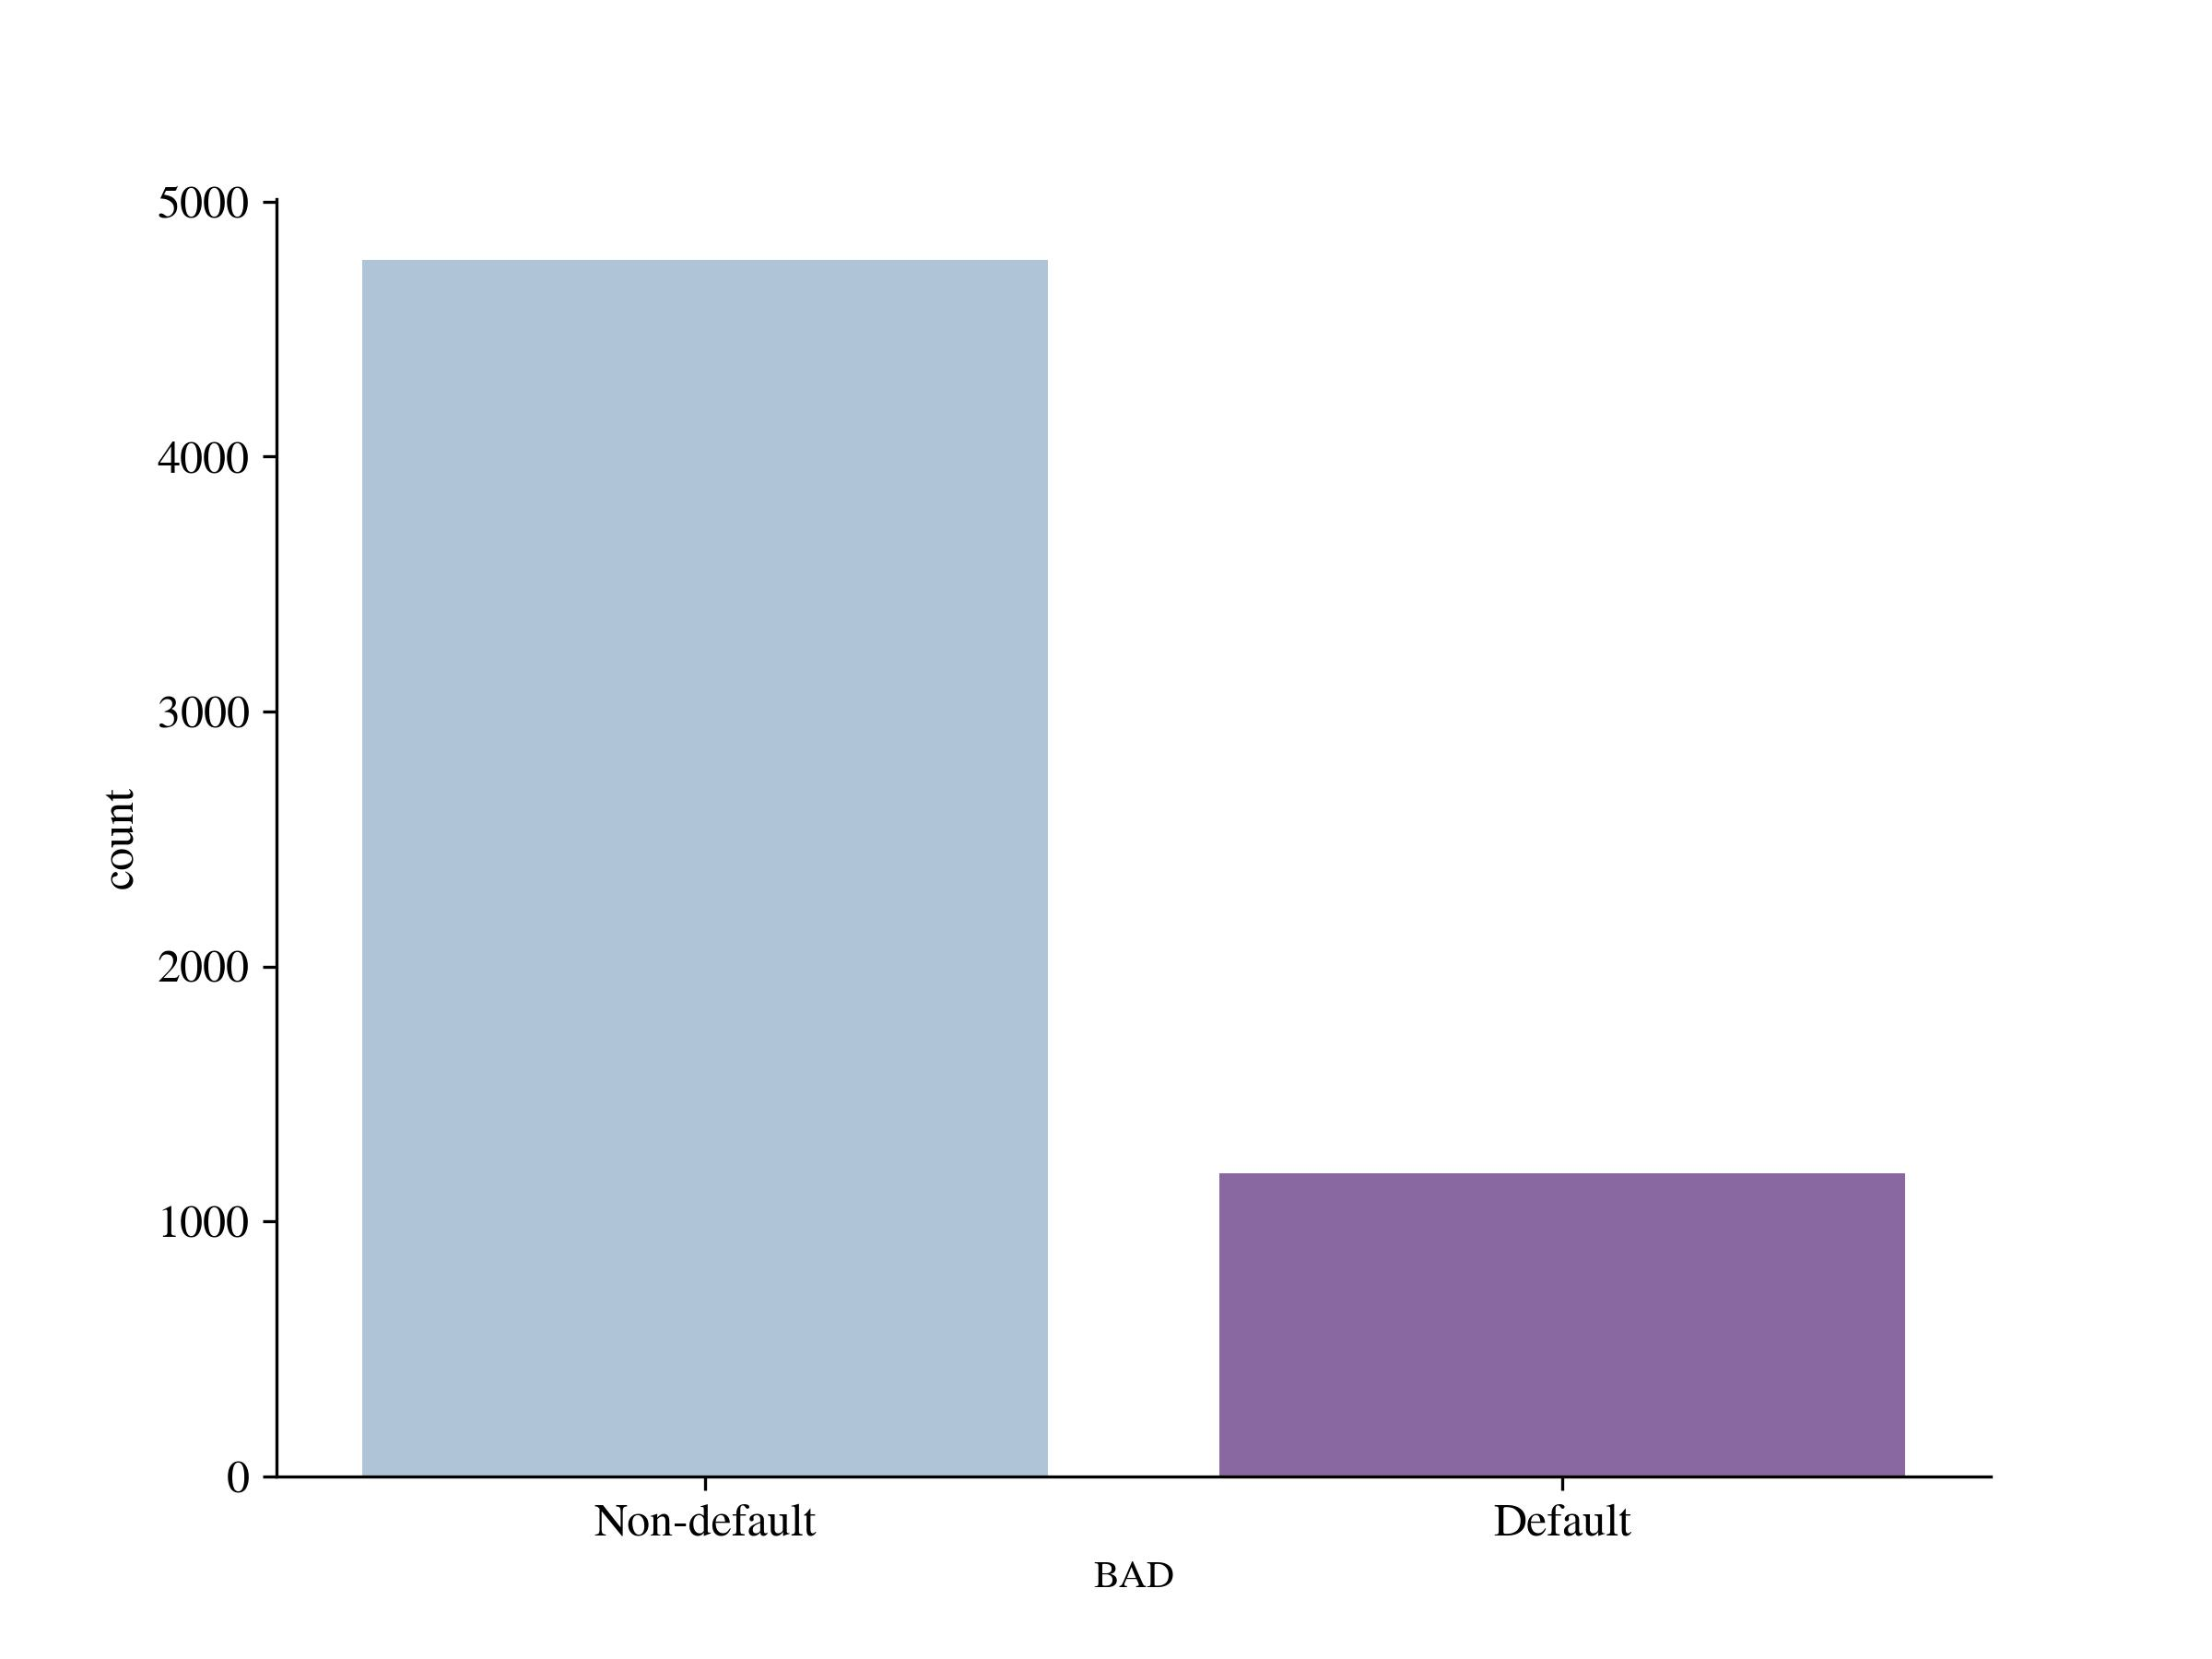
\includegraphics[width=150mm]{Figures/Default_Distribution.jpg}
\end{center}
\begin{center}
    \begin{source}Author's results in Python.\end{source}
    \end{center}
\end{figure}

\subsubsection{Numeric Features' Distribution}
\label{subsubsec:numdist}

With regards to the numeric features, most of the features are positively skewed containing outliers as can be seen in \autoref{fig:boxfeat}, which depicts conditional distribution of numeric features on the default status visualized using boxplots.

All the outliers appear to be valid, i.e., they have not occurred due to data entry errors.
This can be attributed to the fact that all the numeric features are non--negative, thus it is not possible to have negative number of years at present job, negative number of delinquent credit lines, etc. 
Furthermore, the maximum values of given features are not unrealistically high, which further confirms the validity of the outliers.
Nevertheless, the outliers need to be treated since they can biased model's weights or coefficients (in case of logistic regression or neural networks), jeopardize distance calculation (in case of KNN) or in general, they can affect the position and orientation of the decision boundary -- all the reasonings can lead to the model's overfitting and inaccurate and biased predictions.
The outliers' treatment is further described in \autoref{subsec:prep-optbinning}.

With respect to the target variable, we can observe some differences in the distribution shapes of \texttt{DEROG} and \texttt{DELINQ}, which are less skewed and have lower dispersion for non--default cases compared to the default cases.
Since both features indicates a negative information about the delinquency, it is expected that the higher value is, the more likely the loan will end in default.
Referring to the feature \texttt{DEBTINC}, it does not have any extreme values for non--default cases, but it has some extreme values for default cases. We can infer that if the debt--to--income ratio is too high, hence applicant's income is not sufficient to cover his debt, the loan is more likely to end in default.
The assocation between the default status and the numeric features is further investigated in \autoref{subsubsec:target-num-ass}.

\begin{figure}[H]
    \begin{center}
    \caption{Conditional distribution of numeric features}
    \label{fig:boxfeat}
    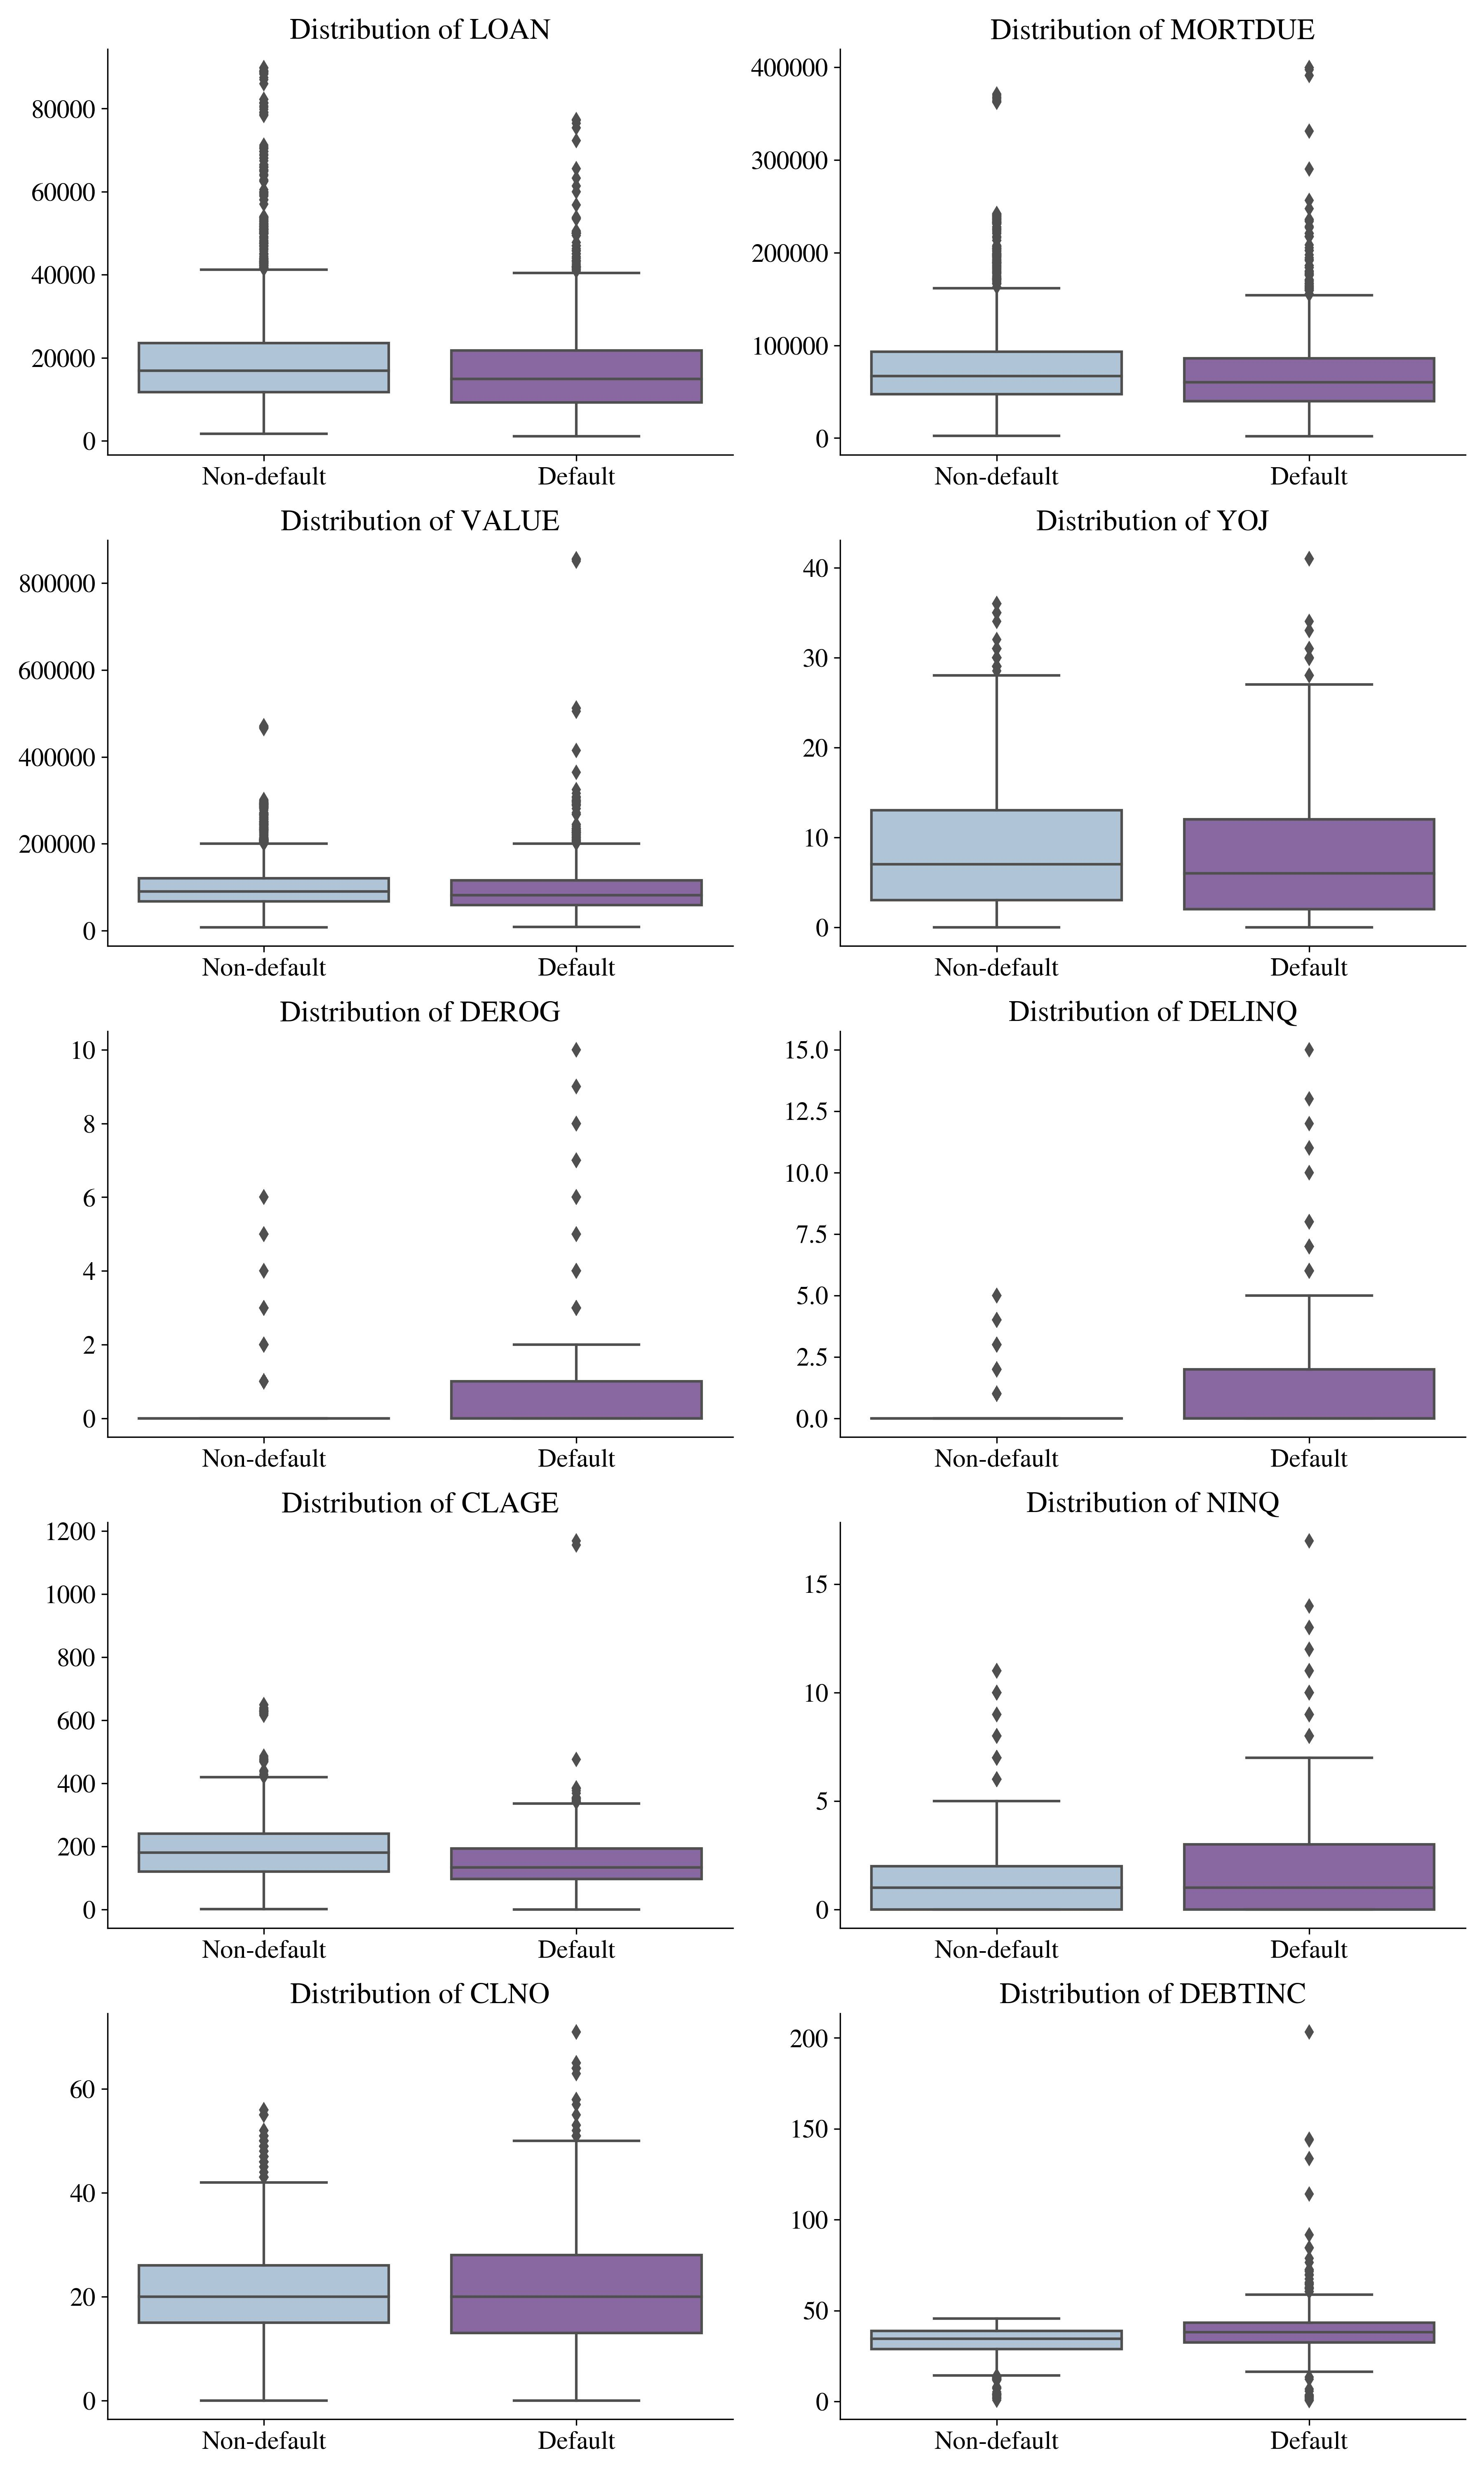
\includegraphics[width=140mm]{Figures/Continuous_Features_Distribution_Boxplots.jpg}
\end{center}
\begin{center}
    \begin{source}Author's results in Python.\end{source}
    \end{center}
\end{figure}

Due to the fact that the boxplots do not capture the missing values occurred in given features, it is also important to inspect the numbers and proportions of missing values in each feature, conditional on the default status.
As can be seen in \autoref{tab:nacont-table}, $n_0$ refers to the number of missing values in given feature for non-default cases, $n_1$ refers to the number of missing values in given feature for default cases.
$N_0$ and $N_1$ refer to the total number non--default cases and default cases respectively, therefore $n_0/N_0$ refers to the proportion of missing values in given feature for non-default cases, and $n_1/N_1$ refers to the proportion of missing values in given feature for default cases.

Pertaining to the feature \texttt{DEBTINC}, we can observe a significant difference in the number of missing values between the default and non-default cases. Out of all defaulted loans, 66.11 \% had missing debt--to--income ratio, whereas only 10.08 \% out of all non-defaulted loans had missing debt--to--income ratio.
Therefore, there could be a strong association between the missing debt--to--income ratio and the default.

Similarly, the table depicts a significant difference with respect to \texttt{VALUE} as 0.15 \% had missing collateral property value out of all non--defaulted loan, and 8.92 \% defaulted loans had missing collateral property value.
It can be inferred that loan applicants who withhold information on their collateral property value or debt-to-income ratio are more likely to default on their loans.
This may be due to negative information that they are trying to conceal, such as an excessively high debt or low income, or a low collateral property value.
Such associations are further investigated in \autoref{subsubsec:target-na-ass}.


\begin{table}[H]
    \small
    \setlength{\tabcolsep}{8pt}
    \renewcommand{\arraystretch}{1.3}
 % define a new column type 'L' for left alignment
    \newcolumntype{R}[1]{>{\raggedleft\arraybackslash}p{#1}} % define a new column type 'R' for right alignment
    \begin{center}
        \caption[Numeric features NA's table]{Numeric features NA's table}\label{tab:nacont-table}
        \begin{tabular}{l R{1cm}R{1cm}|R{1.5cm}R{1.5cm}}
            \toprule
            \textbf{Feature} & \textbf{$n_0$} & \textbf{$n_1$} & \textbf{$n_0/N_0$} & \textbf{$n_1/N_1$} \\
            \midrule
            \hline
            LOAN & 0 & 0 & 0 \% & 0 \% \\

            MORTDUE & 412 & 106 & 8.64 \% & 8.92 \% \\
 
            VALUE & 7 & 105 & 0.15 \% & 8.83 \% \\
   
            YOJ & 450 & 65 & 9.43 \% & 5.47 \% \\

            DEROG & 621 & 87 & 13.02 \% & 7.32 \% \\

            DELINQ & 508 & 72 & 10.65 \% & 6.06 \% \\

            CLAGE & 230 & 78 & 4.82 \% & 6.56 \% \\

            NINQ & 435 & 75 & 9.12 \% & 6.31 \% \\

            CLNO & 169 & 53 & 3.54 \% & 4.46 \% \\

            DEBTINC & 481 & 786 & 10.08 \% & 66.11 \% \\ \hline
            \bottomrule
        \end{tabular}
    \end{center}
    \begin{center}
        \source{Author's results in Python}
    \end{center}
\end{table}


\subsubsection{Categorical Features' Distribution}
\label{subsubsec:catdist}

Pertaining to the categorical features, such dataset has 2 nominal features - \texttt{REASON} and \texttt{JOB}. The following \autoref{fig:catdist} depicts the conditional distribution of categorical features on the default status visualized using barplots.
We can observe that most of the loan applicants applied for a loan because of the debt consolidation and/or their job occupancies were labelled as \texttt{Other}.

Regarding the default status, there does not seem to be a significant difference between the default and non-default cases in terms of relative distribution of \texttt{REASON}.
However, we can observe a slight difference between the default and non-default cases in terms of relative distribution of \texttt{JOB} feature. Particularly, in the categories \texttt{Office}, \texttt{ProfExe} and \texttt{N/A} there is relatively higher proportion of non--default cases than default cases. Therefore, there could be a moderate association between the \texttt{JOB} feature and the default status -- such association is further investigated in \autoref{subsubsec:target-cat-ass}.

\begin{figure}[H]
    \begin{center}
    \caption{Conditional distribution of categorical features}
    \label{fig:catdist}
    \includegraphics[width=140mm]{Figures/Categorical_Features_Distribution.jpg}
\end{center}
\begin{center}
    \begin{source}Author's results in Python.\end{source}
    \end{center}
\end{figure}


\subsection{Association Analysis}
In this subsection, we focus on the association analysis in order to inspect potential relationships between the variables. First, we inspect the association between the default status and the features and aftewards, we check for the association amongst the features themselves.


\subsubsection{Association between default status and numeric features}
\label{subsubsec:target-num-ass}

In order to measure an association between the target variable and the numeric features, we use Point--Biserial correlation which denotes the value of Pearson's product moment correlation between the continuous variable and dichotomous variable \citep{kornbrot2014point}. Such coefficient ranges from -1 to +1.

\begin{equation}\label{eq}
    r_{pb,X} =  \frac{\mu \left( X | Y=1 \right) -\mu \left( X | Y=0 \right)}{\sigma_{X}}\sqrt{\frac{N\left(Y=1\right) \times N\left(Y=0\right)}{N \left(N - 1 \right)}}
\end{equation}

where $\mu \left( X | Y=1 \right)$ and $\mu \left( X | Y=0 \right)$ are the means of given numeric feature $X$ conditional on the default status and non--default status, respectively, $\sigma_{X}$ is the standard deviation of given numeric feature $X$, $N\left(Y=1\right)$ and $N\left(Y=0\right)$ are the numbers of observations with default status and non--default status, respectively, and $N$ is the total number of observation within given feature $X$.


In the following \autoref{tab:pointbi}, we can observe the computed Point-Biserial coefficient for each numeric feature with respect to the default status, including its statistical significance.
As can be seen, features such as \texttt{DEROG}, \texttt{DELINQ} and \texttt{DEBTINC} are moderately and positively association with default status on 1\% statistical significance level.
Thus, we can confirm the findings from \autoref{subsubsec:numdist} regarding the positive associations of the features \texttt{DEROG}, \texttt{DELINQ} and \texttt{DEBTINC} with the default status.
It can be deemed and inferred that such features may be important predictors within modelling.

    \begin{table}[H]
        \small
        \setlength{\tabcolsep}{8pt}
        \renewcommand{\arraystretch}{1.3}
        \begin{center}
            \caption[Point--Biserial Correlation table]{Point--Biserial Correlation table}\label{tab:pointbi}
            \begin{tabular}{@{} l r @{\hspace{1cm}} l @{}}
        \toprule
        \textbf{Feature} & \textbf{Coefficient} & \textbf{Significance}\\
        \midrule
        \hline
       
        LOAN & -0.075  & ***\\
       
        MORTDUE & -0.048  & ***\\
       
        VALUE & -0.030  & ** \\
        
        YOJ & -0.060  & *** \\
      
        DEROG & 0.276 & *** \\
     
        DELINQ & 0.354 & *** \\
        
        CLAGE & -0.170 & *** \\

        NINQ & 0.175 & *** \\

        CLNO & -0.004 & \\

        DEBTINC & 0.200 & *** \\
        \hline
        \bottomrule
        \end{tabular}
        \end{center}

        \begin{center} % Center the source
    
            \footnotesize{$^{*}$: $p<0.10$, $^{**}$: $p<0.05$, $^{***}$: $p<0.01$}

        \end{center}
            \begin{center}

            \source{Author's results in Python}
        \end{center}
    \end{table}

\subsubsection{Association between default status and categorical features}
\label{subsubsec:target-cat-ass}

For measuring a relationship's strength between the dichotomous and categorical variables, we use Cramer's V which ranges from 0 to 1 and is defined as:

\begin{equation}\label{eq}
		CV_{X} = \sqrt{\frac{\chi^{2}}{N\left(k-1\right)}}
		\end{equation}

As expected based on findings in \autoref{subsubsec:catdist}, according to the following \autoref{tab:cramer-v}, the association between the default status and \texttt{REASON} is really weak as the Cramer's V is close to zero.
On the other hand, we can observe slightly stronger association of \texttt{JOB} with default status as some of its categories, namely \texttt{Office}, \texttt{ProfExe} and \texttt{N/A}, showed a higher proportion of non--default cases compared to the default cases. 
Note both \texttt{REASON}'s and \texttt{JOB}'s associations with default status are statistically significant on 1\% significance level.
Although statistical significance is important, it does not guarantee that a feature is a strong predictor of the target variable. Ultimately, the performance metrics of the model are what determine the usefulness of a feature in predicting the target variable.


        \begin{table}[H]
            \small
            \setlength{\tabcolsep}{8pt}
            \renewcommand{\arraystretch}{1.3}
            \begin{center}
                \caption[Cramer's V Association table]{Cramer's V Association table}\label{tab:cramer-v}
                \begin{tabular}{@{} l r @{\hspace{1cm}} l @{}}
            \toprule
            \textbf{Feature} & \textbf{Coefficient} & \textbf{Significance}\\
            \midrule
            \hline
            REASON & 0.038  & ***\\
            JOB & 0.120  & ***\\
            \hline

            \bottomrule
        \end{tabular}
    \end{center}
    \begin{center} % Center the source
        \footnotesize{$^{*}$: $p<0.10$, $^{**}$: $p<0.05$, $^{***}$: $p<0.01$}
    \end{center}
        \begin{center}
        \source{Author's results in Python}
    \end{center}
\end{table}


\subsubsection{Association between default status and missing values}
\label{subsubsec:target-na-ass}

Since the loan data contains missing values, it is deemed appropriate to check whether the missing values are associated with the default status as well. One way how to deal with the measurement, is to encode the feature into a binary variable where 1 indicates a missing value occurrence and 0 otherwise.

For measuring a strength of association between the two binary variables, we use Phi coefficien which is defined as:

\begin{equation}\label{eq}
    \phi_{X} = \sqrt{\frac{\chi^{2}}{n}}
    \end{equation}

In line with the finding regarding the \texttt{DEBTINC} and \texttt{VALUE} in \autoref{subsubsec:numdist}, as shown in \autoref{tab:phi-target}, we can observe a strong and statistically significant association between the missing debt--to--income and default status, respectively a moderate and statistically significant association between the missing collateral property value and the default status. Hence, we can expect such indicators will be the main drivers in a default prediction.

    \begin{table}[H]
        \small
        \setlength{\tabcolsep}{8pt}
        \renewcommand{\arraystretch}{1.3}
        \begin{center}
            \caption[Phi Correlation Coefficient table]{Phi Correlation Coefficient table}\label{tab:phi-target}
            \begin{tabular}{@{} l r @{\hspace{1cm}} l @{}}
        \toprule
        \textbf{Feature} & \textbf{Coefficient} & \textbf{Significance}\\
        \midrule
        \hline
        LOAN & 0.000  & \\
        \hline
        MORTDUE & 0.003  & \\
        \hline
        VALUE & 0.254  & *** \\
        \hline
        REASON & 0.004 & \\
        \hline
        JOB & 0.064 & *** \\
        \hline
        YOJ & 0.056  & *** \\
        \hline
        DEROG & 0.070 & *** \\
        \hline
        DELINQ & 0.061 & *** \\
        \hline
        CLAGE & 0.030 & ** \\
        \hline
        NINQ & 0.039 & *** \\
        \hline
        CLNO & 0.018 & \\
        \hline
        DEBTINC & 0.547 & *** \\
        \bottomrule
        \end{tabular}
        \end{center}

        \begin{center} % Center the source
    
            \footnotesize{$^{*}$: $p<0.10$, $^{**}$: $p<0.05$, $^{***}$: $p<0.01$}

        \end{center}
            \begin{center}

            \source{Author's results in Python}
        \end{center}
    \end{table}

\subsubsection{Missing Values Association}
    \begin{figure}[H]
        \begin{center}
        \caption{Nullity dendrogram}
        \label{fig:supply}
        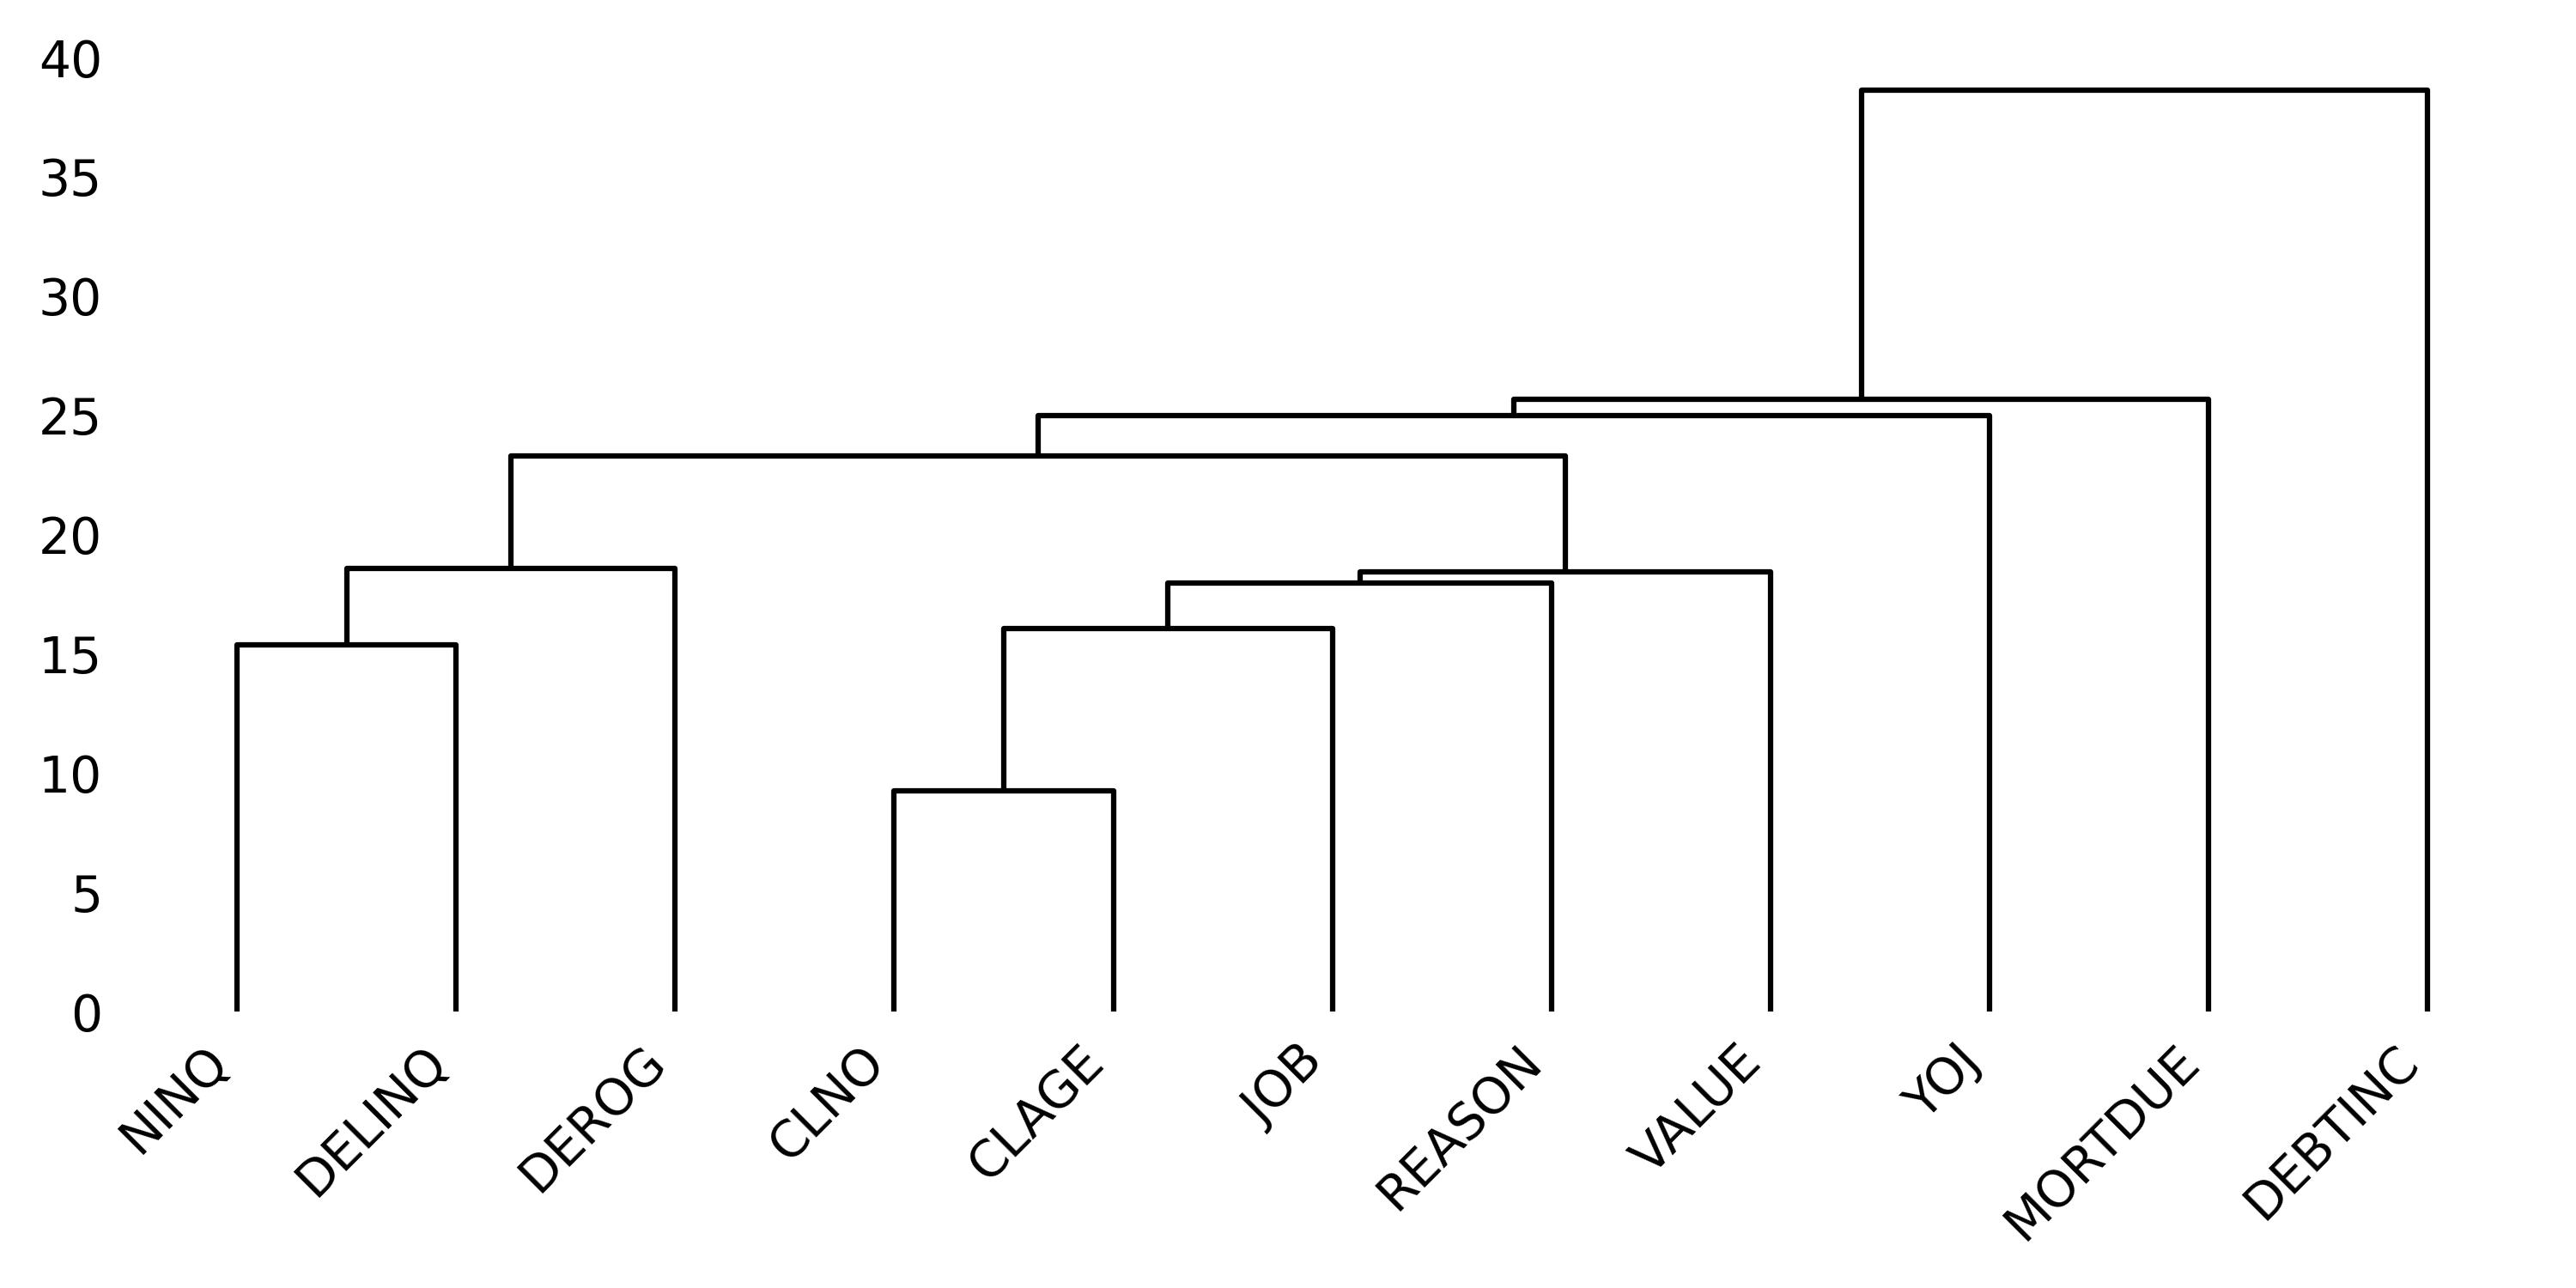
\includegraphics[width=150mm]{Figures/NA_Dendrogram.jpg}
    \end{center}
    \begin{center}
        \begin{source}Author's results in Python.\end{source}
        \end{center}
    \end{figure}
    

\subsubsection{Multicolinearity Analysis}

ADD contigency table for REASON and JOB.

To measure the correlation between the numeric features, one would use Pearson correlation coefficient. However, such measure is very sensitive to outliers and assumes normal distribution of variables as well as the linear relationship between the variables. Therefore, we use Spearman correlation coefficient instead, which is a nonparametric measure of the association between two continuous variables. It is defined as:

\begin{equation}\label{eq}
	\rho_{spearman} = 1 - \frac{6 \sum_{i=1}^{n} d_{i}^{2}}{n \left(n^{2}-1\right)}
	\end{equation}


In the \autoref{fig:spearmancorr}, we can observe a very strong correlation between the \texttt{MORTDUE} and \texttt{VALUE} features. Such multicolinearity can cause problem in predictions na model's overfitting. Therefore, a feature selection is recommended - such selection is further described in \autoref{subsec:feature-selection}.

    \begin{figure}[H]
        \begin{center}
        \caption{Spearman Correlation Matrix}
        \label{fig:spearmancorr}
        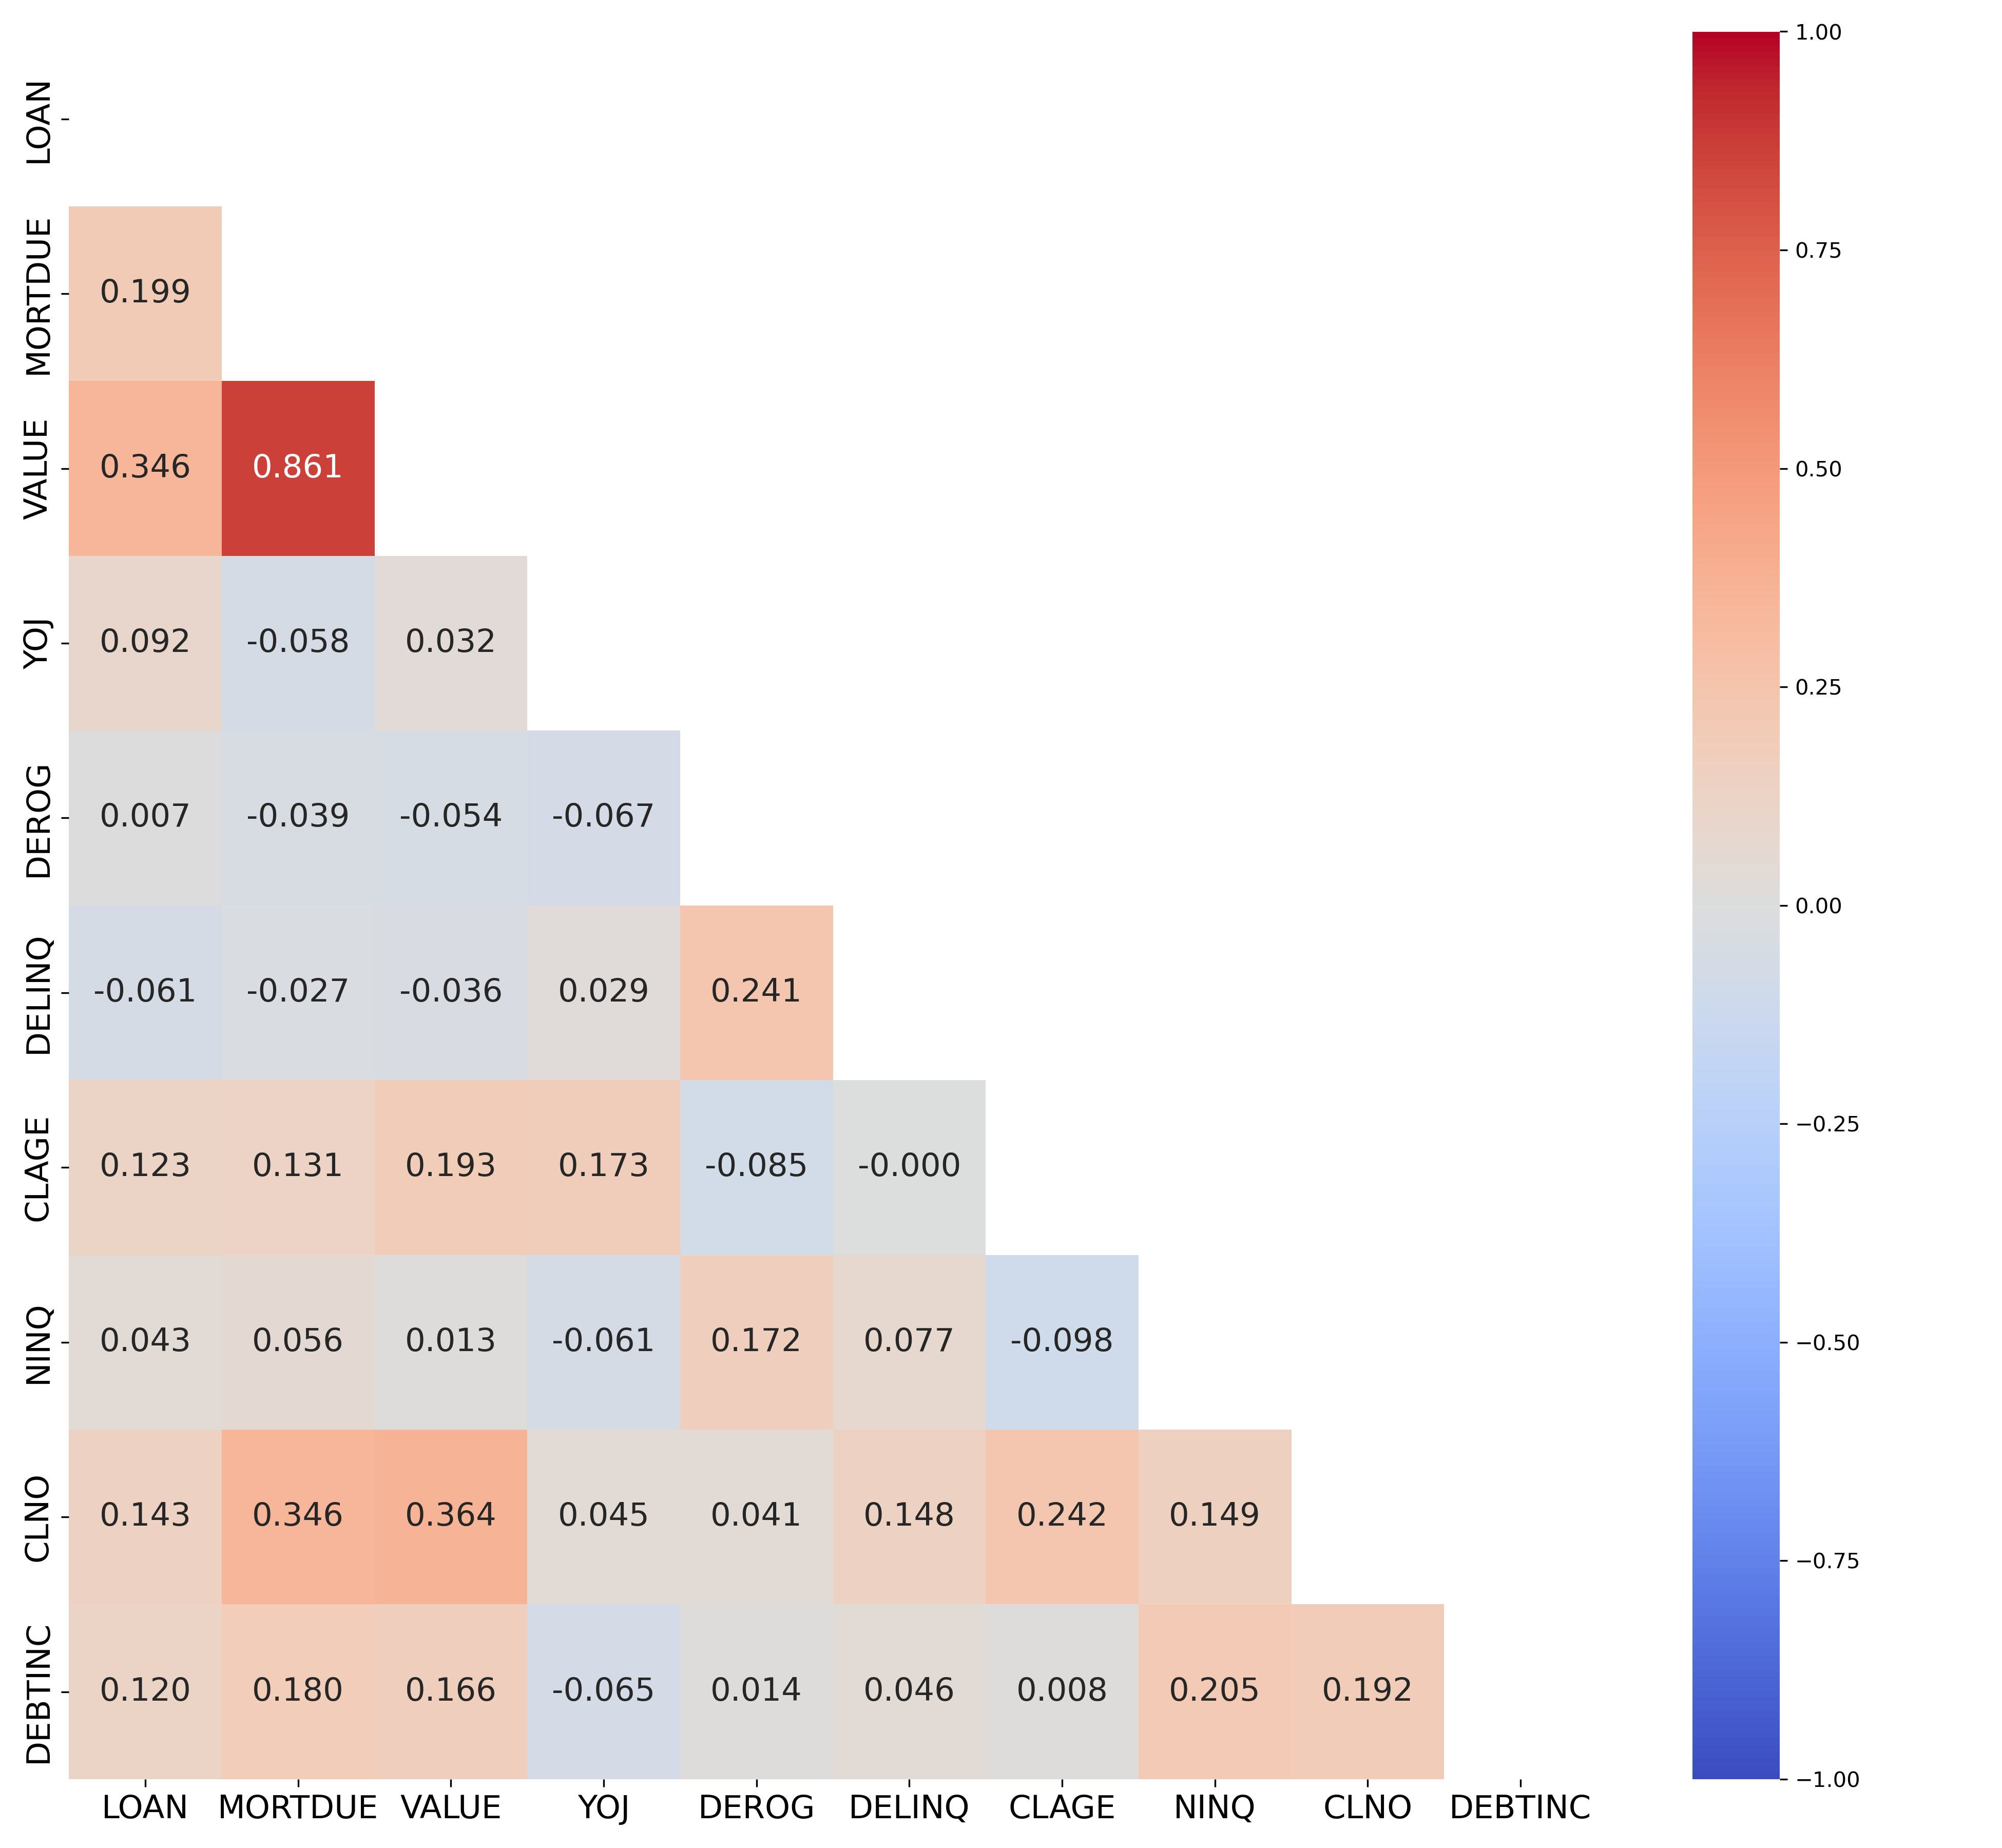
\includegraphics[width=150mm]{Figures/Spearman_Correlation_Matrix_Continuous_Features.jpg}
    \end{center}
    \begin{center}
        \begin{source}Author's results in Python.\end{source}
        \end{center}
    \end{figure}

\section{Data Preprocessing}
\subsection{Data Split and ADASYN Oversampling}
\label{subsec:data-split-ADASYN}
\subsection{Optimal Binning and WoE Encoding}
\label{subsec:prep-optbinning}
\section{Modelling}
\subsection{Hyperparameter Bayesian Optimization}
\subsection{Forward Sequential Feature Selection}
\label{subsec:feature-selection}
\subsection{Model Selection}
\subsection{Model Building}
\section{Model Evaluation}
\subsection{Confusion Matrix}
\subsection{Metrics Scores}
\subsection{ROC Curve}
\subsection{Learning Curve}
\subsection{SHAP Values}
\section{Machine Learning Deployment}
\subsection{Final Model Building}


Itemization and Environments

Many people use simple n-dash in many occasions -- like this --, where however typographic convention---it looks a bit strange at first sight---requires m-dash.
Text text text text text text \citet{Haufler2006}. 

Text text text text text text \citet{Wells2001}. Let us describe the following animals:

\begin{description}
\item[Item 1] Text.
\item[Item 2] Text.
\end{description}

See what Edmund Burke said about the duties of a Member of Parliament (Speech To The Electors Of Bristol At The Conclusion Of The Poll, November 3, 1774):

\begin{quotesmall}
It ought to be the happiness and glory of a representative to live in the strictest union, the closest correspondence, and the most unreserved communication with his constituents. 
Their wishes ought to have great weight with him; their opinion, high respect; their business, unremitted attention.
It is his duty to sacrifice his repose, his pleasures, his satisfactions, to theirs; and above all, ever, and in all cases, to prefer their interest to his own.
But his unbiased opinion, his mature judgment, his enlightened conscience, he ought not to sacrifice to you, to any man, or to any set of men living.
These he does not derive from your pleasure; no, nor from the law and the constitution.
They are a trust from Providence, for the abuse of which he is deeply answerable.
Your representative owes you, not his industry only, but his judgment; and he betrays, instead of serving you, if he sacrifices it to your opinion.
\end{quotesmall}

Text text text text.

\begin{listi}
	\item The first item, the first item, the first item, the first item, the first item, the first item,
	\item and the second item.
\end{listi}

\begin{lista}
	\item The first item, the first item, the first item, the first item, the first item, the first item, 
	\item and the second item.
\end{lista}

TText text text text text text \citet{Blomstrom2003}. 